\documentclass[svgnames,11pt]{beamer}
\input{/home/tof/Documents/Cozy/latex-include/preambule_commun.tex}
\input{/home/tof/Documents/Cozy/latex-include/preambule_beamer.tex}
%\usepackage{pgfpages} \setbeameroption{show notes on second screen=left}
\author[]{Christophe Viroulaud}
\title{Exercices plus court chemin\\correction}
\date{\framebox{\textbf{Archi 16}}}
%\logo{}
\institute{Terminale - NSI}

\begin{document}
\begin{frame}
    \titlepage
\end{frame}
\section{Exercice 1}
\begin{frame}
    \frametitle{Exercice 1}

    \begin{center}
        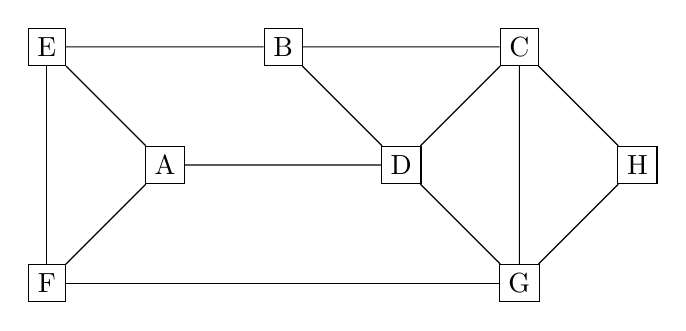
\begin{tikzpicture}[scale=1.5]
            \node[draw] (A) at (1,1) {A};
            \node[draw] (B) at (2,2) {B};
            \node[draw] (C) at (4,2) {C};
            \node[draw] (D) at (3,1) {D};
            \node[draw] (E) at (0,2) {E};
            \node[draw] (F) at (0,0) {F};
            \node[draw] (G) at (4,0) {G};
            \node[draw] (H) at (5,1) {H};

            \draw (A)--(F);
            \draw (A)--(E);
            \draw (E)--(F);
            \draw (A)--(D);
            \draw (E)--(B);
            \draw (F)--(G);
            \draw (D)--(B);
            \draw (B)--(C);
            \draw (D)--(C);
            \draw (D)--(G);
            \draw (G)--(C);
            \draw (G)--(H);
            \draw (H)--(C);
        \end{tikzpicture}

        \vspace{1em}
        \begin{tabular}{|*{8}{c|}}
            \hline
            A & B      & C      & D      & E      & F      & G      & H      \\
            \hline
            0 & \infty & \infty & \infty & \infty & \infty & \infty & \infty \\
            \hline
            0 & \infty & \infty & 1 (A) & 1 (A) & 1 (A) & 2 (F) & 3 (G) \\
            \hline
            0 & 2 (D) & 2 (D) & 1 (A) & 1 (A) & 1 (A) & 2 (F) & 3 (G) \\
            \hline
            0 & 2 (D) & 2 (D) & 1 (A) & 1 (A) & 1 (A) & 2 (F) & 3 (G) \\
            \hline
        \end{tabular}
    \end{center}

\end{frame}
\begin{frame}
    \frametitle{}

    \begin{itemize}
        \item RIP: nombre de sauts entre deux routeurs,
        \item OSPF: coût d'une liaison.
    \end{itemize}

\end{frame}
\begin{frame}
    \frametitle{Bellman-Ford}

    \begin{center}
        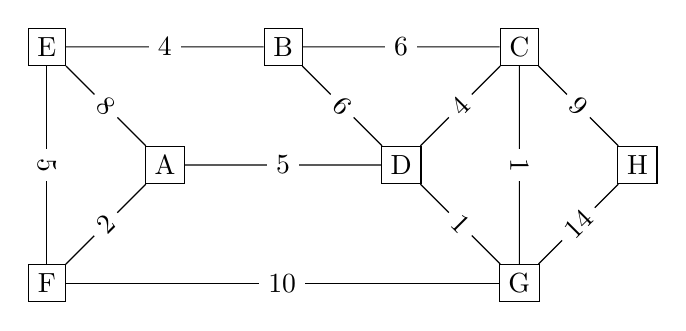
\begin{tikzpicture}[scale=1.5]
            \node[draw] (A) at (1,1) {A};
            \node[draw] (B) at (2,2) {B};
            \node[draw] (C) at (4,2) {C};
            \node[draw] (D) at (3,1) {D};
            \node[draw] (E) at (0,2) {E};
            \node[draw] (F) at (0,0) {F};
            \node[draw] (G) at (4,0) {G};
            \node[draw] (H) at (5,1) {H};

            \draw (A)--(F) node[sloped, midway, fill=white]{2};
            \draw (A)--(E) node[sloped, midway, fill=white]{8};
            \draw (E)--(F) node[sloped, midway, fill=white]{5};
            \draw (A)--(D) node[sloped, midway, fill=white]{5};
            \draw (E)--(B) node[sloped, midway, fill=white]{4};
            \draw (F)--(G) node[sloped, midway, fill=white]{10};
            \draw (D)--(B) node[sloped, midway, fill=white]{6};
            \draw (B)--(C) node[sloped, midway, fill=white]{6};
            \draw (D)--(C) node[sloped, midway, fill=white]{4};
            \draw (D)--(G) node[sloped, midway, fill=white]{1};
            \draw (G)--(C) node[sloped, midway, fill=white]{1};
            \draw (G)--(H) node[sloped, midway, fill=white]{14};
            \draw (H)--(C) node[sloped, midway, fill=white]{9};
        \end{tikzpicture}

        \vspace{1em}
        \begin{tabular}{|*{8}{c|}}
            \hline
            A & B      & C      & D      & E      & F      & G      & H      \\
            \hline
            0 & \infty & \infty & \infty & \infty & \infty & \infty & \infty \\
            \hline
            0 & \infty & \infty & \textbf{5 (A)} & \textbf{8 (A)} & \textbf{2 (A)} & \textbf{6 (D)} & \textbf{20 (G)} \\
            \hline
            0 & \textbf{11 (D)} & \textbf{7 (G)} & 5 (A) & \textbf{7 (F)} & 2 (A) & 6 (D) & \textbf{16 (C)} \\
            \hline
            0 & 11 (D) & 7 (G) & 5 (A) & 7 (F) & 2 (A) & 6 (D) & 16 (C) \\
            \hline
        \end{tabular}
    \end{center}

\end{frame}

\begin{frame}
    \frametitle{Dijkstra}

    \begin{center}
        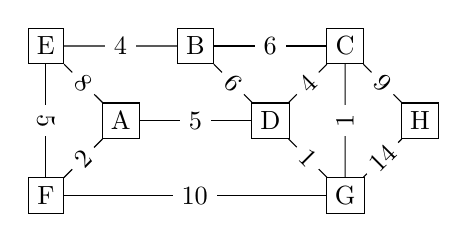
\begin{tikzpicture}[scale=0.95,transform shape]
            \node[draw] (A) at (1,1) {A};
            \node[draw] (B) at (2,2) {B};
            \node[draw] (C) at (4,2) {C};
            \node[draw] (D) at (3,1) {D};
            \node[draw] (E) at (0,2) {E};
            \node[draw] (F) at (0,0) {F};
            \node[draw] (G) at (4,0) {G};
            \node[draw] (H) at (5,1) {H};

            \draw (A)--(F) node[sloped, midway, fill=white]{2};
            \draw (A)--(E) node[sloped, midway, fill=white]{8};
            \draw (E)--(F) node[sloped, midway, fill=white]{5};
            \draw (A)--(D) node[sloped, midway, fill=white]{5};
            \draw (E)--(B) node[sloped, midway, fill=white]{4};
            \draw (F)--(G) node[sloped, midway, fill=white]{10};
            \draw (D)--(B) node[sloped, midway, fill=white]{6};
            \draw (B)--(C) node[sloped, midway, fill=white]{6};
            \draw (D)--(C) node[sloped, midway, fill=white]{4};
            \draw (D)--(G) node[sloped, midway, fill=white]{1};
            \draw (G)--(C) node[sloped, midway, fill=white]{1};
            \draw (G)--(H) node[sloped, midway, fill=white]{14};
            \draw (H)--(C) node[sloped, midway, fill=white]{9};
        \end{tikzpicture}

        \begin{tabular}{|*{8}{c|}}
            \hline
            A & B      & C      & D      & E      & F      & G      & H      \\
            \hline
            0 & \infty & \infty & \infty & \infty & \infty & \infty & \infty \\
            \hline
            0 & \infty & \infty & \textbf{5 (A)} & \textbf{8 (A)} & \textbf{2 (A)} & \infty & \infty \\
            \hline
            \cellcolor{gray}  & \infty & \infty & 5 (A) & \textbf{7 (F)} & 2 (A) & \textbf{12 (F)} & \infty \\
            \hline
            \cellcolor{gray}  & \textbf{11 (D)} & \textbf{9 (D) }& 5 (A) & 7 (F) & \cellcolor{gray} & \textbf{6 (D)} & \infty \\
            \hline
            \cellcolor{gray}  & 11 (D) & \textbf{7 (G)} & \cellcolor{gray} & 7 (F) & \cellcolor{gray} & 6 (D) & \textbf{19 (G)} \\
            \hline
            \cellcolor{gray}  & 11 (D) & 7 (G) & \cellcolor{gray} & 7 (F) & \cellcolor{gray} & \cellcolor{gray} & \textbf{18 (C)} \\
            \hline
            \cellcolor{gray}  & 11 (D) & \cellcolor{gray} & \cellcolor{gray} & 7 (F) & \cellcolor{gray} & \cellcolor{gray} & 16 (C) \\
            \hline
            \cellcolor{gray}  & 11 (D) & \cellcolor{gray} & \cellcolor{gray} &\cellcolor{gray}  & \cellcolor{gray} & \cellcolor{gray} & 16 (C) \\
            \hline
            \cellcolor{gray}  & \cellcolor{gray} & \cellcolor{gray} & \cellcolor{gray} &\cellcolor{gray}  & \cellcolor{gray} & \cellcolor{gray} & 16 (C) \\
            \hline
            \cellcolor{gray}  & \cellcolor{gray} & \cellcolor{gray} & \cellcolor{gray} &\cellcolor{gray}  & \cellcolor{gray} & \cellcolor{gray} & \cellcolor{gray} \\
            \hline
        \end{tabular}
        visités: A - F - D - G - C - E - B - H
    \end{center}

\end{frame}
\section{Exercice 2}
\begin{frame}
    \frametitle{Exercice 2}
    \begin{center}
        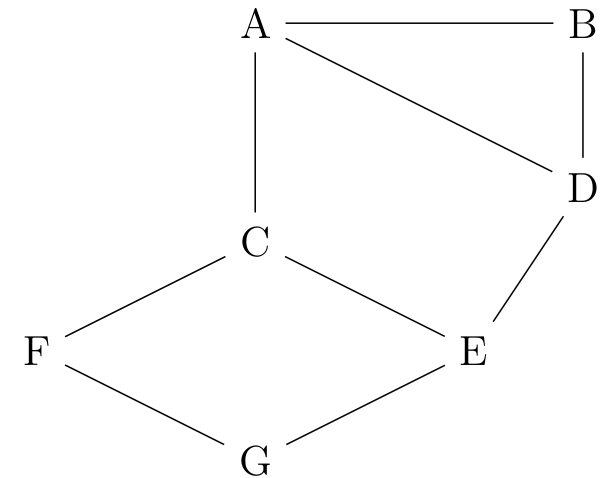
\includegraphics[width=4cm]{ressources/exo-bac.png}
    
        \begin{tabular}{|*{8}{c|}}
            \hline
            A & B      & C      & D      & E      & F      & G            \\
            \hline
            0 & \infty      & \infty      & \infty      & \infty      & \infty      & \infty         \\
            \hline
            0 & 1 (A)     & 1 (A)     & 1 (A)     & 2 (C)      & 2 (C)      & 3 (E)         \\
            \hline
        \end{tabular}
    \end{center}

\end{frame}
\begin{frame}
    \frametitle{}

    coût de 5 $\rightarrow$ bande-passante 20Mbit/s

\end{frame}
\begin{frame}
    \frametitle{}

    \begin{center}
        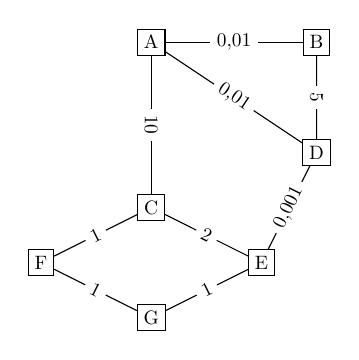
\begin{tikzpicture}[scale=0.7, transform shape]
            \node[draw] (A) at (0,0) {A};
            \node[draw] (B) at (3,0) {B};
            \node[draw] (C) at (0,-3) {C};
            \node[draw] (D) at (3,-2) {D};
            \node[draw] (E) at (2,-4) {E};
            \node[draw] (F) at (-2,-4) {F};
            \node[draw] (G) at (0,-5) {G};

            \draw (A)--(B) node[sloped, midway, fill=white]{0,01};
            \draw (A)--(D) node[sloped, midway, fill=white]{0,01};
            \draw (A)--(C) node[sloped, midway, fill=white]{10};
            \draw (D)--(E) node[sloped, midway, fill=white]{0,001};
            \draw (C)--(E) node[sloped, midway, fill=white]{2};
            \draw (F)--(C) node[sloped, midway, fill=white]{1};
            \draw (F)--(G) node[sloped, midway, fill=white]{1};
            \draw (G)--(E) node[sloped, midway, fill=white]{1};
            \draw (D)--(B) node[sloped, midway, fill=white]{5};
        \end{tikzpicture}
        {\footnotesize
        \begin{tabular}{|*{8}{c|}}
            \hline
            A & B      & C      & D      & E      & F      & G            \\
            \hline
            0 & \infty      & \infty      & \infty      & \infty      & \infty      & \infty         \\
            \hline
            0 & \textbf{0,01 (A)}     & \textbf{10 (A) }    & \textbf{0,01 (A) }    & \infty      & \infty       & \infty        \\
            \hline
            \cellcolor{gray} & 0,01 (A)     & 10 (A)     & 0,01 (A)     & \infty      & \infty     &\infty          \\
            \hline
            \cellcolor{gray} & \cellcolor{gray}    & 10 (A)     & 0,01 (A)     & \textbf{0,011 (D)}   & \infty     &\infty          \\
            \hline
            \cellcolor{gray} & \cellcolor{gray}    & \textbf{2,011 (E)}     &\cellcolor{gray}     & 0,011 (D)   & \infty     & \textbf{1,011 (E)}          \\
            \hline
            \cellcolor{gray} & \cellcolor{gray}    & 2,011 (E)     &\cellcolor{gray}     & \cellcolor{gray}   & \textbf{2,011 (G)}     & 1,011 (E)          \\
            \hline
            \cellcolor{gray} & \cellcolor{gray}    & 2,011 (E)     &\cellcolor{gray}     & \cellcolor{gray}   & 2,011 (G)     & \cellcolor{gray}        \\
            \hline
            \cellcolor{gray} & \cellcolor{gray}    & \cellcolor{gray}    &\cellcolor{gray}     & \cellcolor{gray}   & 2,011 (G)     & \cellcolor{gray}        \\
            \hline
            \cellcolor{gray} & \cellcolor{gray}    & \cellcolor{gray}    &\cellcolor{gray}     & \cellcolor{gray}   & \cellcolor{gray}     & \cellcolor{gray}        \\
            \hline
        \end{tabular}
        }
    \end{center}
\end{frame}
\end{document}